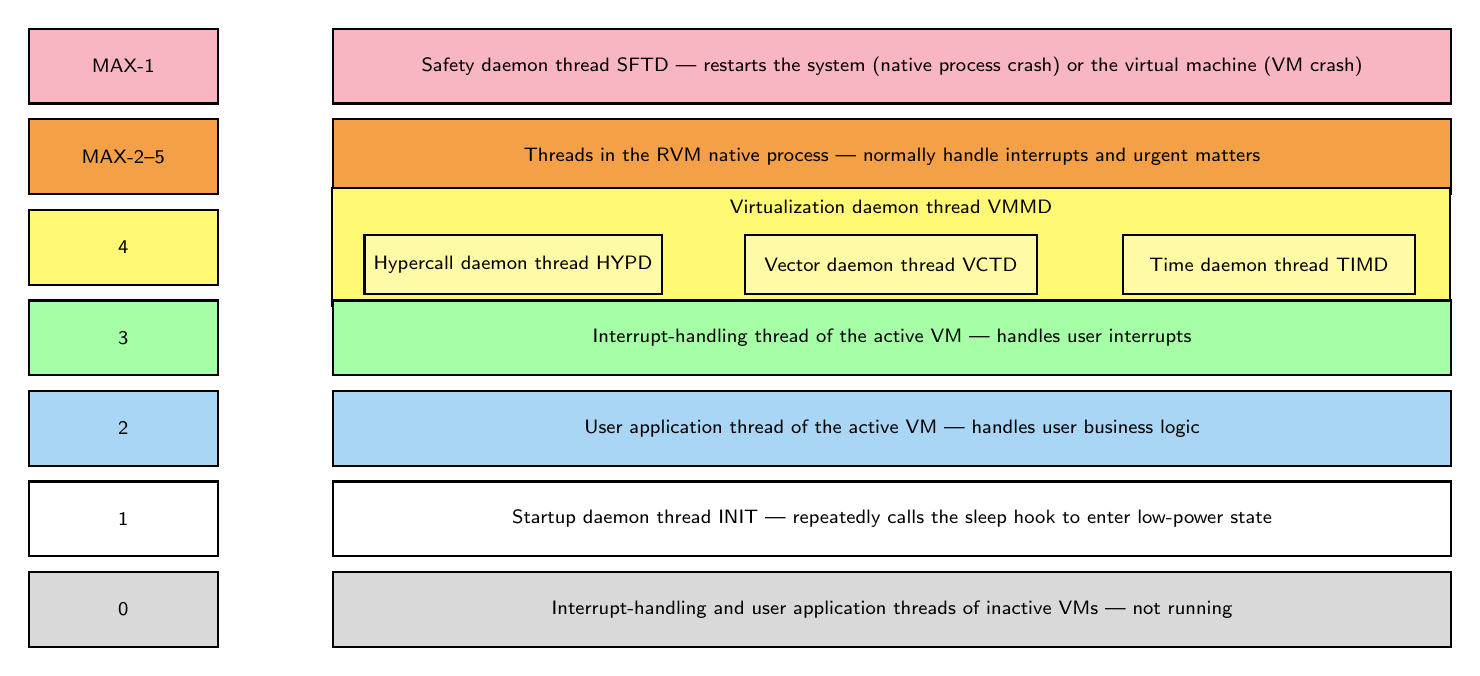
\begin{tikzpicture}[x=1cm,y=1cm,font=\sffamily\scriptsize,
    prio/.style={draw,thick,minimum width=2.4cm,minimum height=0.95cm,align=center},
    bar/.style={draw,thick,minimum height=0.95cm,align=center},
    daemon/.style={draw,thick,fill=yellow!35,minimum height=0.75cm,align=center}]
\definecolor{rvmpink}{RGB}{247,182,194}
\definecolor{rvmblue}{RGB}{169,214,245}
\definecolor{rvmorange}{RGB}{244,160,70}
% Priority rows, top to bottom
\node[prio,fill=rvmpink] (p1) at (0,0) {MAX-1};
\node[bar,fill=rvmpink,minimum width=14.2cm,anchor=west] at (2.65,0) {Safety daemon thread SFTD --- restarts the system (native process crash) or the virtual machine (VM crash)};
\node[prio,fill=rvmorange] at (0,-1.15) {MAX-2--5};
\node[bar,fill=rvmorange,minimum width=14.2cm,anchor=west] at (2.65,-1.15) {Threads in the RVM native process --- normally handle interrupts and urgent matters};
\node[prio,fill=yellow!55] at (0,-2.30) {4};
\draw[thick,fill=yellow!55] (2.65,-1.55) rectangle (16.85,-3.05);
\node at (9.75,-1.78) {Virtualization daemon thread VMMD};
\node[daemon,minimum width=3.7cm] at (4.95,-2.52) {Hypercall daemon thread HYPD};
\node[daemon,minimum width=3.7cm] at (9.75,-2.52) {Vector daemon thread VCTD};
\node[daemon,minimum width=3.7cm] at (14.55,-2.52) {Time daemon thread TIMD};
\node[prio,fill=green!35] at (0,-3.45) {3};
\node[bar,fill=green!35,minimum width=14.2cm,anchor=west] at (2.65,-3.45) {Interrupt-handling thread of the active VM --- handles user interrupts};
\node[prio,fill=rvmblue] at (0,-4.60) {2};
\node[bar,fill=rvmblue,minimum width=14.2cm,anchor=west] at (2.65,-4.60) {User application thread of the active VM --- handles user business logic};
\node[prio,fill=white] at (0,-5.75) {1};
\node[bar,fill=white,minimum width=14.2cm,anchor=west] at (2.65,-5.75) {Startup daemon thread INIT --- repeatedly calls the sleep hook to enter low-power state};
\node[prio,fill=gray!30] at (0,-6.90) {0};
\node[bar,fill=gray!30,minimum width=14.2cm,anchor=west] at (2.65,-6.90) {Interrupt-handling and user application threads of inactive VMs --- not running};
\end{tikzpicture}
